% Este é o arquivo principal, onde o seu trabalho é gerado
% Se tiver dúvidas, leia os comentários ou as referências
% da biblioteca ABNTeX 2.
% Ou também consulte http://aureliocasoni.xyz/latex
\documentclass[12pt,oneside,chapter=TITLE,
    section=TITLE,a4paper,english,brazil,sumario=abnt-6027-2012,]{abntex2}
\tracingoutput
\tracingmacros

% Remove as advertências bizarras de inclusão de pacotes em subpastas. 
\usepackage{silence}
%Disable all warnings issued by latex starting with "You have..."
\WarningFilter{latex}{You have requested package}

\usepackage{include/unigran}

\usepackage[T1]{fontenc}		% Selecao de codigos de fonte.
\usepackage{lastpage}			% Usado pela Ficha catalográfica
\usepackage{indentfirst}		% Indenta o primeiro parágrafo de cada seção.
\usepackage{color}				% Controle das cores

\usepackage{adjustbox}

\usepackage{longtable,ltcaption} % para as tabelas

\usepackage{amssymb}
\usepackage{amsmath}
\usepackage{amsthm}


\usepackage{helvet}			% Usa a fonte Latin Modern			
%\usepackage{lmodern}			% Usa a fonte Latin Modern			
\usepackage[utf8]{inputenc}		% Codificacao do documento (conversão automática dos acentos)
			% Controle das cores
\usepackage{graphicx}			% Inclusão de gráficos
\usepackage{caption}
\usepackage{subcaption}
%\usepackage{subfig}
%\captionsetup[subfigure]{labelfont=rm}
\newcommand{\subfigref}[1]{\hyperref[#1]{Figura~\ref*{#1}}}
\usepackage{float}
\usepackage{url}
\usepackage{multirow}
\usepackage{textcomp}
\usepackage{microtype} 			% para melhorias de justificação
\usepackage{enumerate}
\usepackage{enumitem}
\usepackage{amsmath}
\usepackage{siunitx}

\usepackage{varwidth}
\usepackage{multirow} % Mesclar linhas
\usepackage{microtype} 			% para melhorias de justificação

\usepackage{pdfpages}  
\usepackage{tocloft}                                % Permite alterar a formatação do Sumário
\usepackage{etoolbox}                               % Usado para alterar a fonte da Section no Sumário

\usepackage{lipsum}
\usepackage{rotating}				%Permite usar tabela rotada
\usepackage{float}
% ---
% Pacotes de citações
% ---
%\usepackage[brazilian,hyperpageref]{backref}	 % Paginas com as citações na bibl
\usepackage[alf, abnt-etal-text=emph, abnt-dont-use-etal=yes, bibjustif]{abntex2cite}	         % Citações padrão ABNT

\usepackage{include/url6023} % remove os <> entre a Url, segundo a nova versão da NBR 6023:2018
% se, em uma futura atualização completa do Abntex, isso causar erros na geração da Url, pode comentar na linha acima
% https://github.com/abntex/abntex2/issues/210


% ---

% --- 
% CONFIGURAÇÕES DE PACOTES
% --- 

% ---
% Configurações do pacote backref
% Usado sem a opção hyperpageref de backref
%\renewcommand{\backrefpagesname}{Citado na(s) página(s):~}
% Texto padrão antes do número das páginas
%\renewcommand{\backref}{}
% Define os textos da citação
% \renewcommand*{\backrefalt}[4]{
% 	\ifcase #1 %
%		Nenhuma citação no texto.%
%	\or
%		Citado na página #2.%
%	\else
%		Citado #1 vezes nas páginas #2.%
%	\fi}%
% ---
%configuração para a lista de quadros
%%% nome para ser usado no sumário

%%%%%%%%%%%%%%%%%%%%%%%%%%%%%%%%%%%%
%Informação para configuração das figuras
\newcommand{\source}[1]{\caption*{Fonte: {#1}} }
% ---
% Informações de dados para CAPA e FOLHA DE ROSTO
% Preencha com bastante atenção!
% ---
% Título do seu trabalho
\titulo{Título da tese ou dissertação}

% Nome(s) do(s) autor(es) do seu trabalho. Se tiver mais de um, separe-os com \\
% Se não for uma monografia, coloque o seu RGM
\autor{Nome do candidato}

% Exemplo de dois autores - Ponha um \\ entre eles e remova os %
% \autor{JOSÉ CARLOS ALVES RGM - 99.603\\
% FULANO - RGM xx.XXX}

% Local, nem precisa mexer
\local{Duque de Caxias - RJ}

% Ano do seu trabalho
\data{20aa}

%\renewcommand{\orientadorname}{Orientadora:} %caso seja mulher, apague o % no início da linha

% Nome do seu orientador
\orientador{Nome do Orientador(a)}

%\renewcommand{\coorientadorname}{Coorientadora:} %caso seja mulher
% Coorientador, se não tiver, coloque um % antes dessa linha
\coorientador{Nome do Coorientador(a)}
 
\tipotrabalho{[Dissertação de Mestrado][Tese de doutorado][Monografia para Qualificação ao Doutorado]}
% Se não for monografia, coloque Pré-Projeto, Relatório, Trabalho, etc

% O preambulo deve conter o tipo do trabalho, o objetivo, 
% o nome da instituição e a área de concentração 
\preambulo{\imprimirtipotrabalho apresentada ao Programa de Pós-Graduação em [Biotecnologia] [Metrologia] [Metrologia e Qualidade] do Instituto Nacional de Metrologia, Qualidade e Tecnologia como parte dos requisitos para a obtenção do título de [Mestre] [Doutor] em Ciências.}
% ---

\def \b{$\bullet$}


% ----
% Início do documento
% ----
\begin{document} %Não remova esta linha!

% Retira espaço extra obsoleto entre as frases.
\frenchspacing 

% ----------------------------------------------------------
% ELEMENTOS PRÉ-TEXTUAIS
% ----------------------------------------------------------
\pretextual

\pagenumbering{roman}

% ---
% Capa
% ---
\imprimircapa
% ---

% ---
% Folha de rosto
% (se você digitar \imprimirfolhaderosto* indica que haverá a ficha bibliográfica)
% Mas como a ficha é feita depois, não precisa colocar
% ---
\imprimirfolhaderosto
% ---

\include{pre-textuais/ficha-catalografica}
\include{pre-textuais/folha-de-aprovacao}

% Errata, só é aplicado caso haja um erro no seu trabalho
%\include{pre-textuais/errata}


% Os três itens a seguir, são mais usuais se você estiver redigindo sua monografia.
\include{pre-textuais/dedicatoria}
\include{pre-textuais/agradecimentos}
\include{pre-textuais/epigrafe}

% ---
% RESUMOS
% ---
\setlength{\absparsep}{18pt} % ajusta o espaçamento dos parágrafos do resumo

% Inclui os arquivos de resumo
% Usual apenas para monografia, ou se seu professor exigir
% Se não precisar, apague a(s) linha(s) ou coloque um % antes
\include{pre-textuais/resumo}
\include{pre-textuais/abstract}

% ---
% inserir lista de ilustrações
% ---
\pdfbookmark[0]{\listfigurename}{lof}
\listoffigures*
\cleardoublepage
% ---
% inserir lista de quadros
% ---
\pdfbookmark[0]{\listtablename}{lot}
\listofquadros*
\cleardoublepage

% ---
% ---
% inserir lista de tabelas
% ---
\pdfbookmark[0]{\listtablename}{lot}
\listoftables*
\cleardoublepage
% ---

% ---
% insere a lista de algoritmos
% veja o algoritmo de exemplo e as linhas 250 a 275 do arquivo 
% unigran.sty para saber as palavras-chave
% ---
%\imprimirlistadealgoritmos

% ---
% inserir lista de codigos-fonte
% ---
%\imprimirlistadecodigosfonte

% ---
% inserir lista de abreviaturas e siglas
% ---
\input{pre-textuais/siglas.tex}
% ---
% inserir lista de simbolos
% ---
\input{pre-textuais/simbolos}
% ---
% ---
% inserir o sumario
% ---
\pdfbookmark[0]{\contentsnamebookmark}{toc}
\tableofcontents*
\cleardoublepage
% ---

% ----------------------------------------------------------
% ELEMENTOS TEXTUAIS
% ----------------------------------------------------------
\textual

%reconta da primeira página
\pagenumbering{arabic}
\setcounter{page}{1}

% Aqui inclui os capítulos
% Eles estão dentro da pasta capitulos

\chapter{Introdução}
%\thispagestyle{empty}

Este modelo deve ser utilizado para facilitar a elaboração da monografia, particularmente teses e dissertações. Este modelo poderá ser utilizado, com as devidas adaptações, para trabalhos de disciplinas, quando exigido.
Neste documento estão sendo utilizadas as definições conforme a norma técnica ABNT NBR 14724:2011. A definição de tese é:
\begin{citacao}
“documento que apresenta o resultado de um trabalho experimental ou exposição de um estudo científico de tema único e bem delimitado. Deve ser elaborado com base em investigação original, constituindo-se em real contribuição para a especialidade em questão. É feito sob a coordenação de um orientador (doutor) e visa a obtenção do título de doutor, ou similar” (ABNT NBR 14724:2011, item 3.33).
\end{citacao}
A definição de dissertação é a seguinte:
\begin{citacao}
“documento que apresenta o resultado de um trabalho experimental ou exposição de um estudo científico retrospectivo, de tema único e bem delimitado em sua extensão, com o objetivo de reunir, analisar e interpretar informações. Deve evidenciar o conhecimento de literatura existente sobre o assunto e a capacidade de sistematização do candidato. É feito sob a coordenação de um orientador (doutor), visando a obtenção do título de mestre” (ABNT NBR 14724:2011, item 3.10).
\end{citacao}
Trabalho de conclusão de curso de graduação, trabalho de graduação interdisciplinar, trabalho de conclusão de curso de especialização ou aperfeiçoamento tem a seguinte definição.
\begin{citacao}
“documento que apresenta o resultado de estudo, devendo expressar conhecimento do assunto escolhido, que deve ser obrigatoriamente emanado da disciplina, módulo, estudo independente, curso, programa, e outros ministrados. Deve ser feito sob a coordenação de um orientador” (ABNT NBR 14724:2011, item 3.35).
\end{citacao}

A definição de monografia é apresentada na norma técnica ABNT NBR 6023:2018, segundo a qual monografia é um “item não seriado, isto é, item completo, constituído de uma só parte, ou que se pretende completar em um número preestabelecido de partes separadas”. Assim sendo, teses, dissertações e TCC são monografias.

Além de ser um modelo para elaboração da monografia, este documento traz dicas e boas práticas de elaboração de textos técnicos. Parte do conteúdo é de utilização obrigatória, como as regras de ortografia e gramática, e parte é recomendação. Cabe ao autor, em entendimento com o orientador, discernir sobre o que é obrigatório e o que é recomendável.

AVISO IMPORTANTE: este guia somente poderá ser utilizado como modelo se a edição for feita na versão atual e oficial do Word, preferencialmente o Office 365. O uso de versões anteriores poderá desconfigurar o texto. O autor deverá ficar atento aos requisitos de formatação, particularmente listas, sumário e referências cruzadas.

O primeiro capítulo da monografia deve conter os seguintes elementos: motivação para a pesquisa; tema; justificativa; premissas; hipóteses, escopo; e objetivos. Não é necessário que esses elementos sejam separados em seções específicas, exceto os objetivos. Um bom texto introdutório deixa clara a motivação que levou o pesquisador a escolher determinado tema, justificando apropriadamente sua realização. As premissas são afirmações, geralmente embasadas na literatura, nas quais as hipóteses são construídas. Por sua vez, hipóteses\footnote{Pesquisas com hipóteses englobam duas ou mais variáveis que se relacionam apenas de uma entre duas formas: associação entre as variáveis ou interferência entre as variáveis \cite{volpato_dicas_2010}. }  são respostas provisórias a uma ou mais perguntas de pesquisa, que ainda não foram testadas. Vale mencionar que premissas não podem ser falhas, ou seja, falsas. Se forem, toda a pesquisa será invalidada. As hipóteses, por sua vez, podem ou não ser comprovadas ao final da pesquisa. Caso alguma hipótese seja refutada no decorrer da pesquisa fundamentada nos resultados experimentais, a pesquisa continuará válida e a discussão e conclusões deverão retratar esse achado.

O escopo é fundamental constar na introdução. Este elemento delimita o campo de atuação ou abrangência da pesquisa. As premissas, inclusive, devem fazer alusão ou serem fundamentadas no escopo definido para a pesquisa. Por exemplo: o estudo da propagação ultrassônica em um meio (líquido ou gasoso, por exemplo) depende fundamentalmente da amplitude da onda ultrassônica. A partir de uma determinada amplitude e em função das características do meio e da frequência do sinal, pode-se adotar a teoria de propagação linear ou não linear. Portanto, as premissas, incluindo as equações que vão ser utilizadas, dependem do escopo, ou seja, propagação linear ou não linear. Entretanto, se for definido o escopo como propagação linear, mas se forem realizados experimentos com grandes amplitudes, as premissas serão falsas porque o escopo da pesquisa não foi respeitado.

Em alguns casos, a introdução poderá conter parte da revisão bibliográfica, embora este guia proponha um capítulo independente para revisão bibliográfica (ou fundamentação teórica). 
Cabe ao orientador e o discente escolher a melhor forma de introduzir e fundamentar sua monografia. Segundo a norma ABNT NBR 14724, os elementos textuais são divididos apenas como “Introdução”, “Desenvolvimento” e “Conclusão”, ficando a critério do autor a nomenclatura desses elementos. Reforçando, este guia propõe uma estrutura do “Desenvolvimento” composta por “Fundamentação teórica” (ou “Revisão bibliográfica”), “Metodologia” (ou “Materiais e métodos”), “Resultados” e “Discussão”.

\section{MODELO DO WORD}

Para facilitar o emprego deste modelo, foram criados estilos de texto para serem aplicados nas monografias e para facilitarem a uniformização dos textos. A seguir são apresentados alguns dos estilos criados para este modelo:
TEXTO NORMAL: Fonte: (Padrão) Times New Roman, 12 pt, Recuo: Primeira linha:  1 cm, Justificado. Espaçamento entre linhas:  1,5 linhas, Espaço Antes:  6 pt.
CITAÇÃO LITERAL: Fonte: (Padrão) Times New Roman, 11 pt, Recuo: À esquerda: 4 cm, Justificado. Espaçamento entre linhas:  1,5 linhas, Espaço Depois de:  0 pt,
TÍTULO 1: Fonte: Times New Roman, 12 pt, Negrito, Recuo: À esquerda:  0 cm; Deslocamento:  1 cm, Vários níveis + Nível: 1 + Estilo da numeração: 1, 2, 3, … + Iniciar em: 1 + Alinhamento: Esquerda + Alinhado em:  0 cm + Recuar em:  1 cm, Prioridade: 100.
Outros estilos utilizados neste modelo são: FIGURA; FONTE ORG; ILUSTRAÇÃO; QUADRO; REF BIBLIOGRÁFICAS; TABELA; TÍTULO NN; TÍTULO 2; TÍTULO 3.


\section{Paginação}

Todas as folhas, a partir da folha de rosto inclusive, devem ser contadas sequencialmente, mas não numeradas. A Capa não faz  parte desta numeração. Use a funcionalidade “quebra de seção” para separar a capa do restante do texto. Este guia, se usado como modelo, já está com esta formatação.

A numeração é inserida a partir da primeira página da parte textual (“Introdução”), em algarismos arábicos, no canto superior direito da página, a 2 cm da borda superior, ficando o último algarismo a 2 cm da borda direita da página. No caso de o trabalho ser constituído de mais de um volume, deve ser mantida uma única sequência de numeração das folhas, do primeiro ao último volume. Havendo apêndice e anexo, as suas páginas devem ser numeradas de maneira contínua e a paginação deve dar seguimento à do texto principal.

Quando o trabalho for digitado em anverso e verso, a numeração das páginas deve ser colocada sempre no canto superior externo, ou seja, no anverso no canto superior direito e no verso no canto superior esquerdo.


\section{Objetivo}

Toda pesquisa deve ter um objetivo principal ou geral. O objetivo geral pode ser detalhado em objetivos específicos. Observe que os objetivos específicos fazem parte do objetivo principal. Não são, portanto, outros objetivos distintos. Não utilize o termo “objetivos secundários” pois transmite a impressão de serem pouco relevantes, o que não é o caso. O objetivo geral caracteriza de forma resumida a finalidade do projeto, descrito em um único parágrafo. Ele deve expressar de forma clara qual é a intenção (finalidade) daquele projeto de pesquisa que descreve e delimitar qual será o escopo do trabalho.

Uma pesquisa com muitos objetivos não é uma pesquisa objetiva! Portanto, selecione entre 3 e 6 objetivos específicos. Vale mencionar que cada objetivo específico deve contemplar uma ou algumas etapas do desenvolvimento do projeto. Os objetivos específicos para serem alcançados precisam ter um método ou metodologia, recursos para serem alcançados, devem gerar um resultado (entrega) e devem ser discutidos apropriadamente ao final do trabalho.

Os objetivos devem ser iniciados por verbo. Veja a seguir alguns exemplos categorizados de verbos que podem ser empregados para iniciarem os objetivos (geral ou específicos).


\begin{itemize}
    \item \underline{Verbos de conhecimento:} associar; calcular; citar; classificar; definir; descrever; distinguir; enumerar; especificar; enunciar; estabelecer; exemplificar; expressar; identificar; indicar; medir; mostrar; nomear; registrar; relacionar; relatar; selecionar.
    \item \underline{Verbos de compreensão:} concluir; descrever; distinguir; deduzir; demonstrar; discutir; explicar; identificar; ilustrar; inferir; interpretar; localizar; relatar; revisar.
    \item \underline{Verbos de aplicação:} aplicar; classificar; estruturar; ilustrar; interpretar; organizar; relacionar.
    \item Verbos de análise: analisar; classificar; categorizar; combinar; comparar; comprovar; constatar; correlacionar; diferenciar; discutir; detectar; descobrir; descriminar; examinar; identificar; investigar; provar; selecionar.
    \item \underline{Verbos de síntese:} sintetizar; combinar; compor; criar; comprovar; deduzir; desenvolver; documentar; explicar; organizar; planejar; relacionar
    \item \underline{Verbos de avaliação:} avaliar; concluir; constatar; criticar; interpretar; julgar; justificar; padronizar; relacionar; selecionar; validar; valorizar.
\end{itemize}


\chapter{Revisão de literatura[Fundamentação teórica]}
\thispagestyle{empty}
Em geral, neste capítulo devem ser apresentadas as bases teóricas da sua pesquisa. O capítulo pode ser denominado “Revisão da literatura” (ou “Revisão bibliográfica”) ou “Fundamentação teórica” (ou “Referencial teórico”) consoante seu conteúdo. O termo “Referencial teórico” também pode ser empregado para denominar este capítulo.

“Fundamentação teórica” ou “Referencial teórico”: traz os conceitos básicos e clássicos de física, tecnológicos etc., necessários à compreensão da dissertação.

“Revisão de literatura” ou “Revisão bibliográfica”: é uma retrospectiva do estado da arte sobre o tema da pesquisa, com o objetivo de situar o leitor sobre a situação atual do tema da pesquisa, bem como as lacunas que ainda demanda desenvolvimento. No caso de “Revisão da Literatura” uma detalhada revisão sistemática da literatura deve ser apresentada. Não deve ser feita uma revisão superficial não sistemática, com seleção discricionária e não justificada dos documentos a serem revisados. Deve ser apresentada a estratégia de busca utilizada na revisão sistemática, compreendendo uma seção deste capítulo.

\section{Estratégia de busca}
Caso o capítulo apresente uma revisão da literatura, a estratégia de busca empregada deve ser detalhada. Devem ser apresentados, no mínimo, os seguintes itens:
\begin{itemize}
    \item Termos de busca (simples e compostos)
    \item Critérios de inclusão e exclusão dos documentos
    \item Bases de busca
    \item Recorte temporal (justificado)
    \item Recorte de conteúdo (justificado)
    \item Recorte de língua dos documentos (justificado)
\end{itemize}

\section{Conceitos}
Todo o texto deve ser escrito atendendo a versão mais atual das normas da ABNT. Este guia é apenas orientativo, sendo que os documentos formais de normas de escrita são as versões atualizadas das normas da ABNT.

\section{Breve histórico}
É possível fazer uma revisão da história do tema ou dos principais conceitos que serão utilizados na monografia. Observe que apenas deve ser apresentado o que for relevante para o seu trabalho. É um erro comum o discente incluir vários conceitos fundamentais desnecessários para a compreensão do seu texto, o que o torna enfadonho e pouco atrativo para o leitor.

\section{Linguagem}
Utilize sempre a norma culta da língua portuguesa. Não use gírias, expressões de baixo calão e, principalmente, utilize ortografia correta. Se houver dúvidas sobre a correta escrita de alguma palavra, procure um dicionário da língua portuguesa reconhecido pela Academia Brasileira de Letras (ABL) ou, preferencialmente, o Vocabulário Ortográfico da Língua Portuguesa (VOLP), disponível no site da ABL (ACADEMIA BRASILEIRA DE LETRAS, 2009).

\subsection{Ortografia}
Naturalmente, a ortografia correta é exigência absoluta. Evite anglicismos ou estrangeirismos a menos que sejam absolutamente necessários. Evite usar palavras em língua estrangeira, a menos que tenham sido incorporados ao VOLP. Caso seja absolutamente necessário utilizar palavras em língua estrangeira, estas devem ser grafadas em itálico, seguido do significado entre parênteses.

%Exemplo de Figura

\begin{figure}[H]% H manda colocar exatamente nessa posição no texto (relativa aos parágrafos anterior e %posterior)
	\centering
 	  \caption{Capa da 5ª edição do Vocabulário Ortográfico da Língua Portuguesa}
		\includegraphics{imagens/capavolp.png}
	\label{fig:capavolp}
  \source{disponível em \url{http://www.academia.org.br/nossa-lingua/vocabulario-ortografico}.}
\end{figure}

Segundo a figura \ref{fig:capavolp}.
\subsubsection{Níveis de indentação}
Evite muitos níveis de indentação. Esse é o quarto nível (modelo Título 4). Embora possa haver outros níveis de indentação, 4 níveis é o máximo recomendado.
\subsection{Gramática e estilo}
Empregue sempre a gramática correta no seu texto. Estilo é uma forma individual de escrita. No gênero literário de escrita técnica, o estilo pode variar entre os autores, mas algum rigor deve ser seguido. Nos parágrafos seguintes serão apresentadas algumas dicas que, se seguidas, não serão criticados pela banca e farão seu texto ser mais atrativo para o leitor.

A seguir são apresentados alguns erros típicos de gramática que não devem ocorrer e algumas expressões ou termos que podem ser escritos por questões de estilo.

\begin{enumerate}[label=\alph*)]

{\bfseries \item  Uso da abreviação “etc.”}

O termo “etc.” é a abreviação da expressão em latim “et cetera”, que significa “e outras coisas”. Como trata-se de uma abreviação, deve terminar com um ponto mesmo que esteja no meio da frase, seguindo-se por letra minúscula na palavra subsequente. Se terminar uma frase, basta o ponto de final de período. Como etc. já traz consigo o “e”, não deve ser escrito “e etc.”, nem tampouco deve ser precedido por vírgula. O uso de vírgula antes do etc. pode ser aceito na gramática moderna, mas a linguagem formal tradicional não a permite. Evite usar vírgula antes do etc. Nunca utilize reticências (“...”) após o etc.

{\bfseries \item  Separar sujeito do predicado em uma oração}

O correto uso de vírgulas num texto técnico não é difícil, mas requer a atenção para algumas regras básicas. Um dos erros mais comuns é separar o sujeito do predicado por vírgulas, o que é um erro. Por exemplo:
“As pesquisas realizadas, indicaram que o resultado foi positivo.”
O sujeito desta frase é “as pesquisas realizadas” e o predicado é “indicaram que o resultado foi positivo”. Assim sendo, não pode ser utilizada vírgula para os separar.

{\bfseries \item  Uso do advérbio “mesmo” como pronome}

Esse é um erro fatal que emporcalha o texto. Infelizmente, uma legislação municipal no Rio de Janeiro (e em alguns outros munícipios) propagou um erro de gramática, nos obrigando a ler: “Antes de entrar no elevador, verifique se o mesmo está parado neste andar”. Nesse caso, o termo “mesmo” traz o sentido de um pronome, que se trata de uma classe gramatical da qual o termo “mesmo” não faz parte. O correto seria escrever “Antes de entrar no elevador, verifique se ele está parado neste andar”.

Dica: sempre que for usar o termo “mesmo” ou “mesma”, verifique se pode ser substituído por “ele”, “ela” ou por outro pronome. Se a frase fizer sentido, então não use “mesmo” mas sim o pronome apropriado.
\item {\bfseries Iniciar frase com “E”}

A conjunção aditiva “e” não deve ser utilizado para iniciar. Conjunções são termos que ligam duas ou mais palavras ou orações das mesmas classes gramaticais. Assim sendo, não é gramaticalmente correto iniciar uma frase com conjunção aditiva.

{\bfseries \item  Uso de “e/ou”}

Esse é um tema um tanto controverso. A norma culta da língua portuguesa prescinde do “e/ou” uma vez que o “ou” é não excludente. Isto é, “ou” é uma disjunção não exclusiva, portanto é equivalente ao “e/ou”. Na norma culta, a disjunção exclusiva é dada pelo “ou ... ou”. Por exemplo, para deixar a entender que um laboratório é exclusivamente de calibração ou exclusivamente de ensaio, a norma culta define que seria escrito assim: “... laboratório ou de ensaio ou de calibração”, ou alguma redação semelhante.

Entretanto, vale mencionar que hoje em dia se aceita o “e/ou” em linguagem cotidiana, portanto se trata de estilo usar ou não. Como sugestão, empregue o “e/ou” apenas em casos que a ausência do “e/” venha a trazer confusão no entendimento do texto. Repetindo: o “ou” na língua portuguesa tem o sentido de não exclusividade, portanto já contempla o sentido do “e/”.

{\bfseries \item  Diferença entre ilustração e tabela}

Tabelas são elementos da estrutura de um texto técnico nas quais as principais informações transmitidas são números. Por outro lado, ilustrações podem ser desenhos, esquemas, fluxogramas, fotografias, gráficos, mapas, organogramas, plantas, quadros, retratos etc. Todos estes elementos podem ser genericamente denominados ilustrações, ou especificamente para cada tipo de ilustração. Cada tipo de elemento deve ser enumerado independentemente por ordem de aparecimento no texto. Embora não sejam elementos obrigatórios, geralmente são inseridas listas de tabelas e de ilustrações. A seguir serão apresentados exemplos de tabela, quadro e figura.




%Exemplo de Tabela
\begin{table}[!ht]
		\centering
		\Caption{Quantidade  de dias dos meses do primeiro semestre do ano.}		
		\IBGEtab{}{
		
		    %\resizebox{15cm}{!}{%
		    \begin{adjustbox}{width=0.7\textwidth,center}
			\begin{tabular}{ccccccc}
		    	\toprule
				JAN & FEV & MAR & ABR & MAI & JUN & JUL \\
				\midrule 
				31 & 28 (ou 29) & 31 & 30 & 31 & 30 & 31\\
				\bottomrule
			\end{tabular}
			\end{adjustbox}
		}{
		}
		\source{elaboração própria}
		\label{tab:exemplo-1}
\end{table}


\begin{table}[h]
\centering
\caption{Cotação do dólar turismo na primeira semana de abril de 2020.}
\label{tab:my-table}
\begin{adjustbox}{width=0.4\textwidth,center}
\begin{tabular}{@{}ccc@{}}
\toprule
          & \multicolumn{2}{c}{Cotação em real} \\ \cmidrule(l){2-3} 
Data      & Compra           & Venda            \\
01ABR2020 & 5,2399           & 5,2404           \\
02ABR2020 & 5,2645           & 5,2651           \\
03ABR2020 & 5,2991           & 5,2997           \\
04ABR2020 & --               & --               \\
05ABR2020 & --               & --               \\
06ABR2020 & 5,2465           & 5,2471           \\
07ABR2020 & 5,2211           & 5,2217           \\ \bottomrule
\end{tabular}
\end{adjustbox}
\source{\url{https://www4.bcb.gov.br} [acessado em 23ABR2020].}
\end{table}

    \begin{quadro}[h!]
        \caption{Nomes, símbolos e grandezas das unidades do Sistema Interamericano de Metrologia.}
        % coloque aqui o seu quadro
        \centering
		\includegraphics{imagens/Quadro grandezas.png}
	    \label{qd:grandezas}
	    \source{BIPM.}
    \end{quadro}
    
    %Exemplo de Figura
    
\begin{figure}[htbp]
    \caption{Exemplo de Figura.}
	\centering
		\includegraphics[scale=1]{imagens/barco.png}
	\source{elaboração própria.}
	\label{fig:barco}
\end{figure}

Observe que tanto tabelas quanto ilustrações (todos os tipos) devem ter a seguinte formatação: antes do elemento deve haver um título composto por “tipo” ou “palavra designativa” que pode ser desenho, esquema, fluxograma, fotografia, gráfico, mapa, organograma, planta, quadro, retrato, figura, imagem etc. A palavra designativa deve ser iniciada por letra maiúscula e demais letras minúsculas, seguida por um número de ordem de ocorrência no texto em algarismos arábicos, sucedido por um travessão ladeado por espaços simples (“ – ”) e seguido da descrição do elemento “título”, finalizando com um ponto simples. Após o elemento deve ser apresentada sua fonte mesmo que seja de elaboração própria. A grafia correta é, por exemplo: “Fonte: elaboração própria.”. “Fonte: adaptado de REFERÊNCIA.”; “Fonte: extraído de REFERÊNCIA.”. Observe que “Fonte” inicia-se por letra maiúscula e demais letras são minúsculas, seguindo-se dois pontos (“:”) e o texto a seguir deve ser iniciado por letras minúsculas, salvo nas classes gramaticais que demandar iniciarem-se por letras maiúsculas, como nomes próprios ou siglas, por exemplo. A apresentação da fonte deve ser finalizada por um ponto simples. As normas da ABNT são omissas quanto ao uso de ponto simples para finalizar a descrição do elemento (tabela ou ilustração). Entretanto, este guia faz uso desta formatação. O autor precisa ficar atento quando a fonte citar um site, pois o uso de ponto ao fina do site pode fazê-lo não ser identificado pelo navegador na internet. O tamanho da letra das descrições das tabelas, ilustrações e fontes é menor que a do corpo do texto. Neste guia, o tamanho do corpo do texto é 12 e destes elementos citados é 11 (ambos Times New Roman).

Quanto à formatação, a tabela não deve ter linhas verticais, a menos que sejam relevantes para melhor apresentar as informações. São obrigatórias três linhas horizontais em uma tabela: a que delimita o topo (ou início) da tabela; a que separa o topo do corpo (ou meio) da tabela; e a linha inferior que delimita o final da tabela. Outras linhas horizontais podem ser necessárias para melhor apresentação das informações, mas são dispensáveis. O documento que rege a elaboração de tabelas é o guia gerado pelo IBGE (IBGE, 1993).

{\bfseries \item  Equações e fórmulas}

Todas as unidades devem ser baseadas na edição atual do Sistema Internacional de Unidades (SI). A seguir é apresentado um modelo para equações e fórmulas. As equações devem ser numeradas sequencialmente ao longo do texto e referenciadas no texto.

\begin{equation}
(x+a)^{n}= \sum_{k=0}^{n}\binom{n}{k}x^{k}a^{n-k}
\label{equexemplo}
\end{equation}




Na equação \ref{equexemplo}, \begin{math}x\end{math} é uma variável, \begin{math}a\end{math} é uma constante, \begin{math}n\end{math} é o expoente, \begin{math}k\end{math} é o contador e \begin{math}\sum\end{math} é o símbolo de somatório.

{\bfseries \item  Separação de capítulos}

Cada capítulo da sua monografia deverá se iniciar em uma página distinta da do capítulo anterior. Para isso, não acrescente linhas em branco ao final do capítulo até o título do capítulo subsequente “pular” para a próxima página. Os editores de texto, incluindo o MS Word, dispõem de uma ferramenta denominada “inserir quebra de página”. Fica muito mais elegante e evita perda de formatação caso alguma linha seja retirada ou inserida no capítulo.

{\bfseries \item  Manter linhas de cabeçalho e títulos com o texto que o sucede}

Um erro infelizmente recorrente é a presença de “linhas soltas” no texto. Por exemplo, se for introduzido uma seção no final de uma página, pode ocorrer que o parágrafo subsequente ao título da seção “pule” para a página seguinte. Para evitar isso, use a ferramenta de edição “Manter com o próximo”, ou outra denominação do seu editor de texto. Assim, caso a formatação do texto seja alterada, automaticamente o título da seção irá acompanhar o parágrafo que a sucede.

A mesma observação vale para títulos de tabelas e ilustrações. Use da ferramenta “Manter com o próximo” para que o título fique sempre acima e na mesma página do elemento que o sucede, assim como o próprio elemento com a descrição da fonte, elemento obrigatório e que deve suceder a tabela ou ilustração.

É importante NÃO ACRESCENTAR LINHAS ENTRE AS DESCRIÇÕES DAS TABELAS E ILUSTRAÇÕES E ANTES DA DESCRIÇÃO DA FONTE.

{\bfseries \item  Uso de advérbios}

Os advérbios são fundamentais para uma boa escrita. O grande problema é usá-lo apropriadamente. Recomenda-se uma revisão do tema em alguma gramática de boa qualidade. Essencialmente, deve-se atentar para alguns vícios de linguagem recorrentes. Advérbios são elementos gramaticais que, estando próximos (“ad”) a um verbo, adjetivo alteram seu significado (incluindo um outro advérbio). Um erro comum é usar o advérbio de lugar “onde” com função distinta da sua proposta. Eis um uso inapropriado do adverbio “onde”: “Eu fiz um experimento semana passada onde os resultados foram favoráveis”. Mais correto seria “... semana passada quando os resultados ...” (advérbio de tempo e não de lugar).

Outro erro comum é usar a locução adverbial “através de” com o sentido de “por meio de”. “Através” tem sentido de atravessar, enquanto “por meio de” é uma locução adverbial de modo, podendo ser substituída por “do seguinte modo” ou “de tal maneira”.

{\bfseries \item  Siglas}

O correto é escrever o nome por extenso e a respectiva sigla em seguida, e não o inverso. Por exemplo: Agência Nacional de Aviação Civil (ANAC); Instituto Nacional de Metrologia, Qualidade e Tecnologia (Inmetro).
É possível usar a sigla em inglês e fazer a tradução na descrição. Por exemplo: Comissão Internacional de Eletrotécnica (IEC, do inglês International Eletrotechnical Commission). A partir desta definição, pode ser utilizada a sigla IEC normalmente.

{\bfseries \item  Plural de siglas}

Gramaticalmente, não está errado escrever siglas no plural, mas é uma questão de estilo. Muitos leitores preferem a forma clássica de representar siglas apenas na sua forma original, isto é, no singular. Por exemplo, “Unidade Organizacional” tem como sigla “UO”. Ao se referir a mais de uma UO, o autor pode optar por escrever UOs ou manter a sigla original UO. O sentido da oração se dará pelo artigo que precederá a sigla ou pela flexão do verbo, conforme seja a construção da oração. Veja os exemplos a seguir:

“A UO tem 50 servidores.”

“A UO terá seu orçamento anual majorado em 10\%.”

“As UO têm 50 servidores cada.”

“As UO terão seus orçamentos anuais majorados em 10\%.”

Não há dúvidas que os dois primeiros exemplos dizem respeito a apenas uma UO, enquanto os outros dois exemplos se referem a mais de uma UO. Portanto não é necessário acrescentar a letra “s” após a sigla para transmitir ao leitor a informação que são mais de uma UO.

Observação importante: é absolutamente errado usar ’s (apóstrofe seguido da letra “s”) para representar plural de sigla. Por exemplo, está errado escrever “UO’s”.

Ainda em relação ao uso de siglas, estas devem vir por extenso no ponto do texto onde aparecem pela primeira vez. Por exemplo: Coordenação Geral de Acreditação (Cgcre).

{\bfseries \item  Plural de símbolos}

Símbolos não têm plural! A observação é importante, inclusive, para símbolos das unidades do SI. Não existe plural de A ou N, que são os símbolos das unidades ampere (grandeza corrente elétrica) e newton (grandeza força). Entretanto, à unidade escrita por extenso deve ser acrescentada a letra “s” para representar seu plural: amperes e newtons.

{\bfseries \item  Use linguagem formal e não coloquial}

Expressões coloquiais como, por exemplo “tipo assim”, “levantar as informações” etc. não devem ser empregadas. O texto fica pobre e não irá satisfazer o leitor. Essas expressões são aceitas em textos literários, naturalmente, mas não em textos técnicos e científicos.

{\bfseries \item  Vícios de linguagem}

Na linguagem vulgar ou coloquial, o uso de determinadas construções gramaticais ou de estilo são admitidas. Entretanto, em textos técnicos isso não é permitido. A seguir são apresentados alguns exemplos mais comuns. O autor da monografia deve estar atento para não cometer esses ou outros vícios de linguagem.
\begin{itemize}
    \item Usar “através” ao invés de “por meio de”. Exemplo: “As medições foram feitas através de um multímetro”. O correto seria “As medições foram feitas por meio de um multímetro” ou “... com uso de ...”.
    \item 	A expressão “período de tempo” está incorreta. “Período” é uma grandeza equivalente a “tempo”.
\end{itemize}

{\bfseries \item  Referências bibliográficas}

A norma ABNT NBR 6023 apresenta como devem ser elaboradas as referências bibliográficas, elemento pós-textual obrigatório. A citação no corpo do texto deve seguir o previsto na ABNT NBR 10520. Apesar de haver algumas formas de se citarem as referências (sistema de chamadas), a preferencial para monografias é “AUTOR-DATA” (veja cláusula 6.1 da ABNT NBR 10520). A manutenção das referências em um texto longo é muito mais simples quando a lista das referências está em ordem alfabética e não em ordem de aparição no texto. Estude as normas ABNT NBR 10520 e ABNT NBR 6023 para citar apropriadamente as referências na monografia.

Vale observar que o capítulo REFERÊNCIAS BIBLIOGRÁFICAS tem o mesmo nível hierárquico das seções principais (INTRODUÇÃO, REVISÃO BIBLIOGRÁFICA, METODOLOGIA, RESULTADOS, DISCUSSÃO e CONCLUSÃO), mas não é numerado.

A lista de referências diz muito sobre a qualidade do artigo. Deve-se evitar citações bibliográficas em português a menos que sejam estritamente necessárias. Normas, por exemplo, é sempre mais aconselhável citar a versão internacional, se houver, ou similar. Nunca cite teses ou dissertações. Uma boa tese ou dissertação terá gerado artigo em períódico. Procure artigos dos autores daquela tese ou dissertação sobre o assunto. Evite ao máximo citar artigos de congressos. Revistas técnicas e científicas são a melhor fonte de bibliografia técnica e acadêmica, preferencialmente com DOI. Livros, cite pouco e apenas os clássicos.

{\bfseries \item  Coesão textual}

Ao escrever, lembre-se que seu texto como um todo deve fazer sentido para o leitor. O autor, num texto dissertativo (ou mesmo numa tese), busca convencer o leitor acerca de um determinado assunto. Por isso, evite ao máximo inserir mudanças repentinas de assunto ao longo do seu texto. Caso seja preciso mudar de assunto numa mesma seção do seu trabalho, faça-o de maneira elegante, como por exemplo por meio da inserção de parágrafos de ligação.

A transição na exposição de ideias ao longo do seu texto deve ser feita com coerência e lógica, de forma que o texto seja coeso (ou contínuo).Na língua portuguesa há elementos que conferem coesão a um texto. Tratam-se de expressões que estabelecem a transição de ideias entre frases e parágrafos, como pronomes, advérbios e conjunções.

    \begin{quadro}[h!]
        \caption{Exemplos de elementos de coesão textual.}
        % coloque aqui o seu quadro
        \centering
		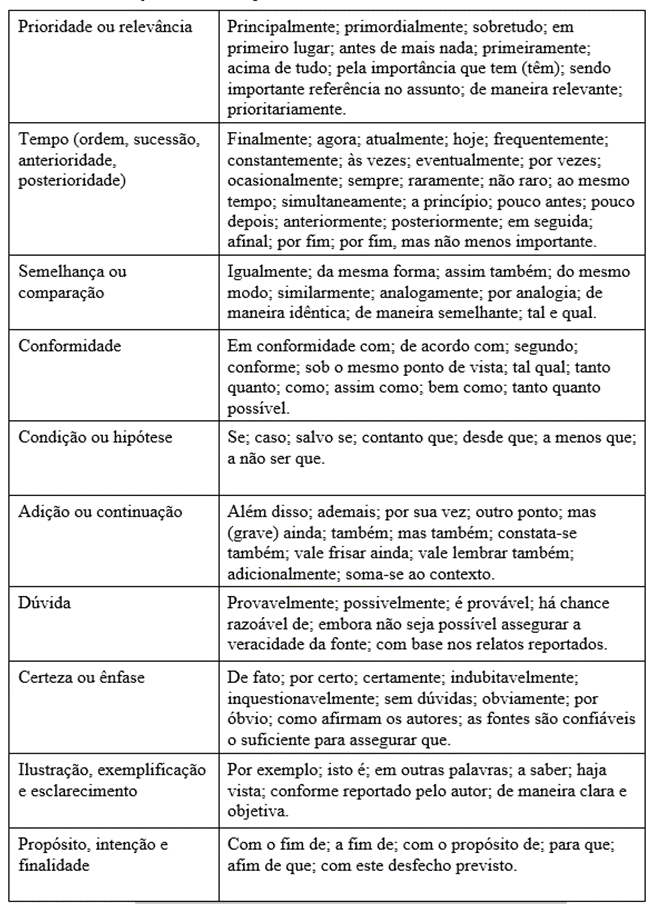
\includegraphics[scale=0.8]{imagens/quadro2.png}
	    \label{qd:grandezas}
	    \source{adaptado de \citeonline{Borges}, com acréscimos de autoria própria.}
    \end{quadro}

\end{enumerate}

\chapter{METODOLOGIA [MATERIAIS E MÉTODOS]}
\thispagestyle{empty}	
\section{CONTEÚDO DESTE CAPÍTULO}
Neste capítulo devem ser apresentados todos os recursos utilizado na sua pesquisa. Se o desenvolvimento do método fez parte da sua pesquisa, então o capítulo pode ser denominado “metodologia”, que significa “estudo dos métodos”. Quando um método foi desenvolvido ou aprimorado, então ele passou por um processo de validação de método, portanto deve ser apresentado neste capítulo.

Há trabalhos que, de fato, fazem um estudo dos métodos, para escolher ou propor algum. Quando isto é feito, precisa estar claro que se trata de metodologia. Este estudo pode ser feito sem o uso de materiais ou aplicação de algum método. Por outro lado (mais comum), não há estudo de métodos. Simplesmente se adota algum método, cuja aplicação prescinde de algum material. Por fim, pode haver a situação onde se discute a metodologia, se escolhe algum método e se aplica através dos materiais necessários.

\section{DESCREVA O QUE USOU E USE O QUE DESCREVEU}
Alguns erros recorrentes presentes em muitas monografias estão na inadequação da apresentação dos materiais e métodos. É importante para uma ótima transmissão de conhecimento descrever TUDO que foi utilizado na sua pesquisa neste capítulo, incluindo aplicativos, recursos humanos, insumos, instrumentos de medição, padrões, equipamentos e acessórios. É considerado erro grave utilizar algum recurso e apresentá-lo em outros capítulos, por exemplo no referencial teórico ou nos resultados. Se policie para não fazer isso.

Muitas vezes o pesquisador propõe um certo método e, no decorrer da pesquisa, termina optando por outra abordagem. Outro fato recorrente é prever o emprego de um determinado instrumento de medição mas utilizar outro semelhante. Caso algo semelhante aconteça, o correto é apresentar ambos instrumentos neste capítulo, eventualmente justificando a troca.

\section{INSTRUMENTOS DE MEDIÇÃO E PADRÕES}

Para apresentar um equipamento ou instrumento de medição, ou mesmo um insumo ou consumível, o correto é a seguinte padronização: “Para realizar a medição XXX foi utilizado um [nome do instrumento, equipamento, padrão ou insumo] modelo [nome, tipo ou descrição do modelo] ([Nome do fabricante], [País]) com as seguintes características: [descrever as principais características]”. Os itens em amarelo devem ser substituídos para cada instrumento e medição, equipamento, padrão ou insumo utilizado na pesquisa.

\section{TRATAMENTO ESTATÍSTICO}

Toda pesquisa de cunho tecnológico demanda algum tratamento estatístico. É obrigatório descrever neste capítulo qual ou quais métodos estatísticos foram empregados para tratamento dos dados ou análise dos resultados. Inclua a probabilidade de abrangências, critérios de aceitação, validação de métodos de medição, testes de hipóteses, técnicas de amostragem, erros máximos admissíveis, tolerâncias e outras limitações estatísticas impostas ou decorrentes do objeto estudado.

\section{USO DE QUESTIONÁRIOS}
Tem sido cada vez mais comum o uso de questionários como instrumentos de pesquisa qualitativa. O uso de questionários requer uma série de cuidados prévios, tanto na elaboração e aplicação do questionário, quanto na análise dos resultados obtidos. Segundo \citeonline{Melo2015}, “a utilização indevida de um questionário, ou um questionário mal formulado, pode resultar na geração de informações equivocadas e causar erros de conclusões, afetando a validade do estudo”.

Os questionários devem ser elaborados de forma criteriosa, estabelecendo uma ligação com o problema de pesquisa, as premissas (ou hipóteses) do estudo, a população a ser pesquisada e os métodos de análises de dados disponíveis. As perguntas que comporão o questionário devem ser claras e objetivas, minimizando ao máximo a possibilidade de vieses por aqueles que irão respondê-las, ou seja, isentas de ambiguidades. Desse modo, perguntas que induzem a resposta (p.ex. “você escova os dentes todos os dias?”), que não trazem a informação pretendida (perguntas que usam pronomes indefinidos: algum, nenhum, todo, outro, muito, pouco, certo, vários, tanto, quanto, qualquer, alguém, ninguém, tudo, outrem, nada, quem, cada, algo) e perguntas que se auto respondem (p.ex. “você prefere que o expediente termine mais cedo?”) não devem ser utilizadas. Deve-se ter atenção também com a lógica na apresentação sequencial das perguntas. \citeonline{Melo2015} acrescentam que perguntas que sugiram ou condicionem a resposta, que possuam conteúdo emocional, que levem o respondente à necessidade de fazer cálculos, que façam alusão a nomes que impliquem em aceitação ou rejeição e que contagiem outras respostas, devem ser evitadas.

É importante frisar que um questionário possui um tamanho ótimo, não devendo ser demasiadamente longo ou curto. Questionários muito longos geram enfado nos respondentes, que ou não o responderão ou passarão a fazê-lo de forma não criteriosa, de qualquer maneira. Questionários muito curtos podem ser insuficientes em termos dos dados necessários para a pesquisa. Nesse ponto, pode-se utilizar a estatística multivariada (nomeadamente a análise multifatorial) a fim de determinar quais são as perguntas importantes a serem mantidas no questionário e quais podem ser removidas.
Ao se optar pelo uso de questionários, o pesquisador deve levar em consideração o tamanho da população e consequentemente da amostra a qual será aplicado este instrumento. Se a população for muito grande, o erro amostral e o tempo na execução da pesquisa devem ser levados em conta antes do seu início. De forma geral, a taxa de retorno dos questionários respondidos no período da pesquisa é baixa.

Outro ponto importante a ser considerado é a confiabilidade do questionário como instrumento de pesquisa. Imagine que você está fazendo uma pesquisa que envolve a medição de pH: você confiaria nos dados obtidos por meio de um medidor de pH que não estivesse devidamente calibrado? Assim também é acontece com os questionários. É necessário que os questionários tenham sua confiabilidade avaliada, o que pode ser feito de diversas maneiras, como por meio do cálculo do alfa de Cronbach, teste-reteste (administrar o questionário duas vezes na mesma pessoa com dado intervalo de tempo), confiabilidade Inter Avaliador (Concordância) (avaliada, por exemplo, por meio do cálculo do Tau de Kendall, correlação interclasse etc.). Alguns fatores podem influenciar a confiabilidade dos questionários. \citeonline{Freitas2005} mencionam três fatores: o número de itens, o tempo de aplicação do questionário e a amostra de avaliadores. 
Por fim, mas não menos importante, ao se elaborar um questionário deve-se avaliar quais os tipos de questões (abertas fechadas ou mistas) bem como qual a escala de avaliação (ordinal, nominal, intervalar etc.) a serem utilizadas. Um tipo de escala muito popular é a escala Likert. A escala Likert típica é uma escala ordinal de 5 ou 7 pontos usada pelos entrevistados para avaliar o grau em que eles concordam ou discordam de uma afirmação.


\chapter{RESULTADOS}
\thispagestyle{empty}
\section{CADA OBJETIVO ESPECÍFICO TEM UM OU MAIS RESULTADOS}
Neste capítulo serão apresentados os resultados da pesquisa sendo relatada na monografia. Vale lembrar que cada objetivo específico deverá ter gerado um ou mais resultados.
Não repita o conteúdo da metodologia neste capítulo. Se houver algum detalhe mal explicado no capítulo de metodologia, ao invés de acrescentar a explicação neste capítulo, corrija o capítulo anterior.
Um breve comentário sobre os resultados pode vir seguido de sua exposição. Cuidado para não entrar em detalhes da discussão, já que esta deve ser realizada no capítulo seguinte.


\chapter{DISCUSSÃO}
\thispagestyle{empty}
Este capítulo é o âmago da monografia. Todos os capítulos são importantes, claro, e devem ter seu conteúdo rigorosamente trabalhado. Entretanto, é neste capítulo que o autor demonstra todo conhecimento adquirido sobre o assunto e o domínio que ele tem sobre os resultados obtidos. Uma boa discussão deixa o leitor ciente que o autor domina o tema e é de fato “proprietário” do conhecimento desenvolvido. Aqui, o autor deve mostrar que as hipóteses foram verificadas e que os objetivos propostos foram atingidos evidenciando sua contribuição ao conhecimento. Esta é a parte da monografia na qual o autor coloca sua opinião sobre o tema e discute com seus pares, por meio do que existe de mais atual na literatura.

Uma boa e completa discussão mescla um debate sobre os seus resultados, realçando pontos fortes e fracos, com uma comparação fundamentada com o que há na literatura. É importante mencionar que não é obrigatório que os resultados da pesquisa sejam idênticos aos reportados na literatura especializada. O autor deve ter senso crítico para interpretar e discutir o que há de semelhante, assim como tranquilamente apontar as diferenças obtidas em relação a outros autores.

A discussão não é uma repetição da revisão bibliográfica, mas é normal usar algumas referências lá citadas para dialogar com os resultados da pesquisa. Uma boa estratégia é discutir os dados obtidos à luz das referências: os dados confirmam a teoria envolvida? Eles sugerem outras interpretações? São sugeridas particularidades?

Há uma questão algoz na redação de monografias de cunho técnico: os capítulos resultados e discussão estarem juntos. É possível, claro. O modelo aqui apresentado se enquadra melhor às pesquisas para as quais há bastante literatura a respeito, o que nem sempre é o caso. Caso o tema tenha literatura importante publicada, a discussão não é sobre os resultados, mas trata-se da comparação dos resultados com a literatura, ou sobre a validação das hipóteses.


\chapter{CONCLUSÃO}
\thispagestyle{empty}

Toda monografia deve terminar com uma conclusão. Neste capítulo não se deve simplesmente repetir trechos da discussão, mas deve ser evidenciada a contribuição da pesquisa para a evolução do conhecimento sobre o tema estudado à luz dos resultados experimentais obtidos.

Embora não seja obrigatório, em geral as conclusões de monografias terminam com um parágrafo elencado assuntos, temas ou abordagens que poderiam servir como trabalhos futuros, quer seja pelo próprio autor ou por outros pesquisadores.
\section{PROPOSTA DE CONTINUIDADE [OPCIONAL]}

Caso haja atividades relevantes relacionados ao trabalho desenvolvido, eles são listados com uma breve explicação, neste capítulo. Afinal, a pesquisa científica é incremental e não se pode esgotar o assunto em um único trabalho de pesquisa.



% ----------------------------------------------------------
% ELEMENTOS PÓS-TEXTUAIS
% Se não tiver, pode apagar tudo até a penúltima linha
% ----------------------------------------------------------
\postextual

% ----------------------------------------------------------

% ----------------------------------------------------------
% Referências bibliográficas
% ----------------------------------------------------------

\bibliography{referencias}

% ----------------------------------------------------------
% Glossário
% ----------------------------------------------------------
% Consulte o manual da classe abntex2 para orientações sobre o glossário.
%\glossary


% Apêndices e anexos
% Segundo a NBR 14724 de dezembro de 2005, a diferença primordial entre Anexo e Apêndice é que o Anexo é um texto ou documento não elaborado pelo autor do Trabalho Científico (TC) (monografia, tese, etc.) e o Apêndice é um texto ou documento elaborado pelo autor do TC
% http://www.portalsaofrancisco.com.br/portugues/anexos-e-apendices
% Não é obrigatório

%\imprimirapendices %insere uma folha com o texto apendices para separar os apendices do restante do texto
\apendices
% Adicione aqui os apendices do seu trabalho
\input{pos-textuais/apendice1}
        
%\imprimiranexos %insere uma folha com o texto anexos para separar os anexos do restante do texto
\anexos
\input{pos-textuais/anexo1}
        
%---------------------------------------------------------------------
% INDICE REMISSIVO
%---------------------------------------------------------------------
% \phantompart
% \printindex
%---------------------------------------------------------------------

%Não apague essa linha
\end{document}
